\documentclass[tikz,10pt,border=.1mm]{standalone}
\usepackage{amsmath,amsfonts,amssymb,siunitx,float,subcaption,setspace,booktabs,diagbox,bm,tikz,structmech,mathtools,tikz-3dplot,pgfplots,url}
\usetikzlibrary{decorations.pathmorphing,shapes.geometric,spy}
\pgfplotsset{compat=1.18}
\newcommand{\balpha}{\mb{\alpha}}
\newcommand{\bbeta}{\mb{\beta}}
\newcommand{\bc}{\mb{c}}
\newcommand{\bd}{\mb{d}}
\newcommand{\be}{\mb{e}}
\newcommand{\beeta}{\mb{\eta}}
\newcommand{\bgamma}{\mb{\gamma}}
\newcommand{\bn}{\mb{n}}
\newcommand{\bq}{\mb{q}}
\newcommand{\bs}{\mb{s}}
\newcommand{\bsigma}{\mb{\sigma}}
\newcommand{\bv}{\mb{v}}
\newcommand{\bvarepsilon}{\mb{\varepsilon}}
\newcommand*{\algoref}[1]{Algorithm~\ref{#1}}
\newcommand*{\ddfrac}[2]{\dfrac{\md{#1}}{\md{#2}}}
\newcommand*{\dev}[1]{\text{dev}\left(#1\right)}
\newcommand*{\diag}[1]{\text{diag}\left(#1\right)}
\newcommand*{\eqsref}[1]{Eq.~(\ref{#1})}
\newcommand*{\figref}[1]{Fig.~\ref{#1}}
\newcommand*{\mb}[1]{\bm{#1}}
\newcommand*{\md}[1]{\mathrm{d}#1}
\newcommand*{\mT}{\mathrm{T}}
\newcommand*{\pdfrac}[2]{\dfrac{\partial{#1}}{\partial{#2}}}
\newcommand*{\sign}[1]{\text{sign}\left(#1\right)}
\newcommand*{\tabref}[1]{Table~\ref{#1}}
\newcommand*{\tr}[1]{\text{trace}\left(#1\right)}
\definecolor{d73027}{HTML}{d73027}
\definecolor{fc8d59}{HTML}{fc8d59}
\definecolor{fee090}{HTML}{fee090}
\definecolor{e0f3f8}{HTML}{e0f3f8}
\definecolor{91bfdb}{HTML}{91bfdb}
\definecolor{4575b4}{HTML}{4575b4}
\begin{document}\footnotesize
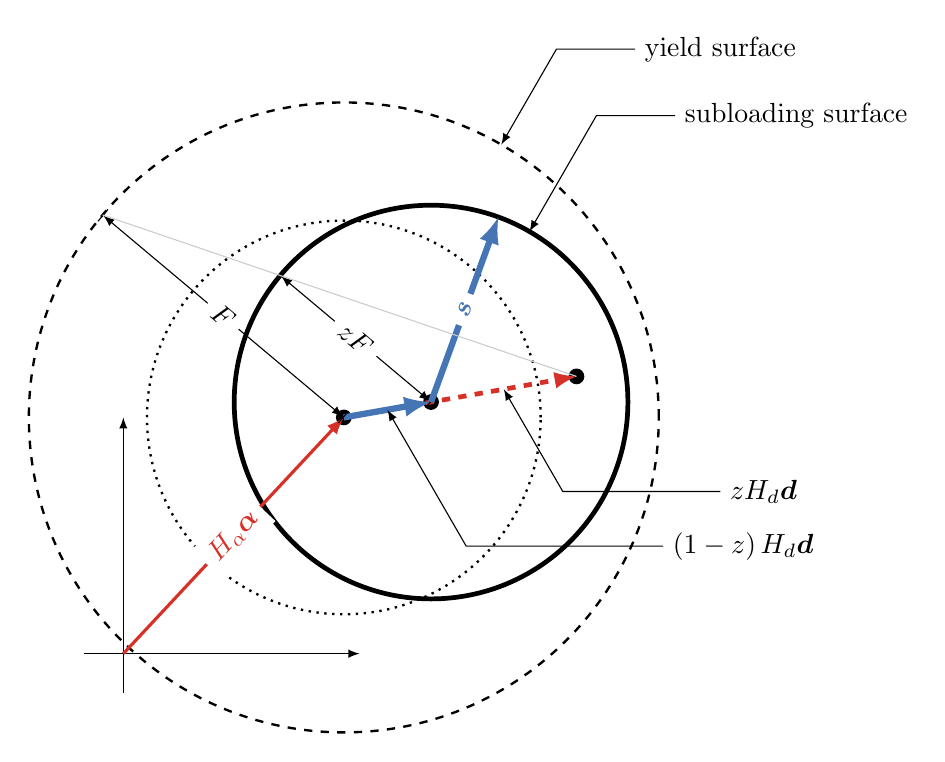
\begin{tikzpicture}[>=latex]
    \newcommand{\FF}{4}
    \newcommand{\SF}{2.5}
    \draw[->](-.5,0)--(3,0);
    \draw[->](0,-.5)--(0,3);
    \coordinate(A)at(2.8,3);
    \coordinate(B)at($(A)+(10:3)$);
    \coordinate(C)at($(B)!\SF/\FF!(A)$);
    \node[fill=black,circle,inner sep=0,minimum size=2mm]at(A){};
    \node[fill=black,circle,inner sep=0,minimum size=2mm]at(B){};
    \node[fill=black,circle,inner sep=0,minimum size=2mm]at(C){};
    \draw[dashed,draw,line width=.3mm](A)circle(\FF);
    \draw[dotted,draw,line width=.3mm](A)circle(\SF);
    \draw[draw,line width=.6mm](C)circle(\SF);
    \draw[->,d73027,line width=.4mm](0,0)--(A)node[midway,fill=white,sloped]{$H_\alpha\balpha$};
    \draw[->,d73027,dashed,line width=.6mm](A)--(B);
    \draw[->,4575b4,line width=.8mm](A)--(C);
    \draw[|<->|](A)--++(140:\FF)node[midway,fill=white,sloped]{$F$};
    \draw[|<->|](C)--++(140:\SF)node[midway,fill=white,sloped]{$zF$};
    \draw[->,4575b4,line width=.8mm](C)--++(70:\SF)node[midway,fill=white,sloped]{$\bs$};
    \draw[<-]($(A)+(60:\FF)$)--++(60:1.4)--++(1,0)node[right,fill=white]{yield surface};
    \draw[<-]($(C)+(60:\SF)$)--++(60:1.7)--++(1,0)node[right,fill=white,align=left]{subloading surface};
    \draw[<-]($(C)!.5!(B)$)--++(-60:1.5)--++(2,0)node[right,fill=white]{$zH_d\bd$};
    \draw[<-]($(A)!.5!(C)$)--++(-60:2)--++(2.5,0)node[right,fill=white]{$\left(1-z\right)H_d\bd$};
    \draw[black!20]($(A)+(140:\FF)$)--(B);
\end{tikzpicture}
\end{document}